\documentclass{beamer}
\usepackage[english]{babel}
\usepackage{calc}
\usepackage[absolute,overlay]{textpos}
\usepackage{graphicx}
\usepackage{subfig}
\usepackage{amsmath}
\usepackage{amsfonts}
\usepackage{amsthm}
\usepackage{mathtools}
\usepackage{comment}
\usepackage{MnSymbol,wasysym}
\usepackage{bm}
\usepackage{cancel}

\setbeamertemplate{navigation symbols}{} % remove navigation symbols
%\mode<presentation>{\usetheme{tud}}

% BIB SETTINGS
\usepackage[backend=bibtex,firstinits=true,maxnames=30,maxcitenames=20,url=false,style=authoryear]{biblatex}
\bibliography{bibfile}
\setlength\bibitemsep{0.3cm} % space between entries in the reference list
\renewcommand{\bibfont}{\normalfont\scriptsize}
\setbeamerfont{footnote}{size=\tiny}
\renewcommand{\cite}[1]{\footnote<.->[frame]{\fullcite{#1}}}

\DeclarePairedDelimiter{\norm}{\lVert}{\rVert} 

\usepackage{graphicx}
\usepackage{amsmath}
\usepackage{amssymb}
%\usepackage{amsmath,amssymb,lmodern}
\usefonttheme[onlymath]{serif}
\usepackage[absolute,overlay]{textpos}

\usepackage{xcolor}
\setbeamertemplate{caption}[numbered]
%\renewcommand{\figurename}{\c{S}ekil}

\DeclareMathOperator{\atantwo}{atan2}

\DeclareMathOperator{\arctantwo}{arctan2}

\definecolor{RowColorOdd}{rgb}{0.914,0.914,0.953}
\definecolor{RowColorEven}{rgb}{1,1,1}

\usepackage{booktabs} % Allows the use of \toprule, \midrule and \bottomrule in tables

\usepackage{etoolbox}
\usepackage{ragged2e}

\apptocmd{\frame}{}{\justifying}{}

\usepackage{textpos}

\def\uncl{\column{1.1\textwidth}} % Full column page width
\def\unclh{\column{0.5\textwidth}} % Half column page width

\usepackage{media9}

\def\ls{\vspace{.8em}} % Line skip
\def\lss{\vspace{.4em}} % Smaller line skip
\def\uncl{\column{1.1\textwidth}} % Full column page width




\title[]{Parameter Identification and State Estimation of an Battery by Using Second Order Equivalent Circuit Model}
\institute[]{}
\author{\.{I}smail \c{C}a\u{g}da\c{s} Y{\i}lmaz}
\date[Apr 2021]{Apr 23, 2021}

\begin{document}
{
\setbeamertemplate{footline}{\usebeamertemplate*{minimal footline}}
\frame{\titlepage}
}

{\setbeamertemplate{footline}{\usebeamertemplate*{minimal footline}}

}

\begin{frame}
	\frametitle{Contents of the Presentation}
	\tableofcontents
\end{frame}

\section{Introduction}
\begin{frame}
	\begin{block}

	\frametitle{Introduction}
		
	For advanced battery management system (BMS) of electric vehicles (EVs)
	\begin{itemize}
		\item Accurate identification of the key state parameters
		\item State of Charge (SOC) estimation method 
	\end{itemize}	
	\vspace{5mm}
	
	Providing an nearly accurate model and SOC framework is of a great significant in 
	\begin{itemize}
		\item Real-time control of battery
		\item High performance operation 
		\item Diagnosis and Prognosis of a battery behavior
	\end{itemize}
	\end{block}	
		
\end{frame}

\begin{frame}
	
	\frametitle{Introduction}
	
	The knowledge of the internal battery parameters is mainly
	required for
	
	\begin{enumerate}
		\item Estimation of the energy losses in the battery during the operation
		
		\vspace{3mm}
		
		\item SOC estimation based on electrical models
		\vspace{2mm}
		
		\item Prediction of the available power of the battery
	\end{enumerate}  

\end{frame}

\section{Equivalent Second-Order Circuit Model (ECM)}

\begin{frame}
	\begin{block}
		
	\frametitle{Equivalent Second-Order Circuit Model (ECM)}
		
		Second-order RC model has the moderate precision and is more
		suitable for the voltage estimation of battery cell.
		
		\begin{figure}
			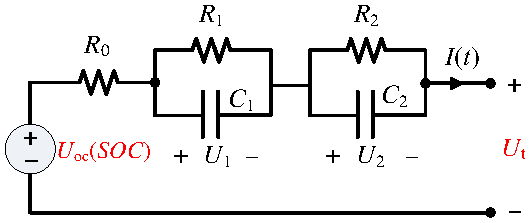
\includegraphics[scale=0.90]{images/Schematic_diagram_of_the_second_order_RC_model.pdf}
			\vspace{-2mm}
			\caption{Schematic diagram of the second-order RC model.}
		\end{figure}
		
	\end{block}	
	
	where $R_{0}=R_{\Omega}$ is ohmic resistances. $R_{1}$ and $C_{1}$ electro-chemical polarization RC parameters. $R_{2}$ and $C_{2}$ represents the concentration polarization RC parameters.
	
\end{frame}

\begin{frame}
	\frametitle{Dynamic Equations of the Second Order ECM}
	The electrical behavior of the second-order RC battery model:
	
	\begin{subequations} 
		\label{eqn:electrical_behavior_of_the_proposed_model}
		\begin{align} \dot{U}_{1}(t) &= -\frac{1}{R_{1}C_{1}}U_1(t) + \frac{1}{C_1}I(t) \\ 
			\dot{U}_{2}(t) &= -\frac{1}{R_{2}C_{2}}U_2(t) + \frac{1}{C_2}I(t) \\ 
			U_{t}(t) &= U_{oc}(SOC)(t) - {U}_{1}(t) - {U}_{2}(t) - I(t)R_{0} 
		\end{align} 
	\end{subequations}	
	
	Mathematical relations involving SOC in continuous time domain:
	\begin{equation}
		\label{eqn:SOC_in_continious_time}
		SOC(t) = SOC(t_{0}) - \frac{1}{Q}\int_{t_{0}}^{t}\eta I(\tau)d\tau~~ \text{or}~~ \dot{SOC(t)} = -\frac{\eta I(t)}{Q}
	\end{equation}
	in discrete time
	
	\begin{equation}
		\label{eqn:SOC_in_discrete_time}
		SOC[k+1] = SOC[k] - \bigg(\frac{\eta T}{Q}\bigg)I[k] \
	\end{equation}
	
\end{frame}

\begin{frame}
	\frametitle{The LTI State Space Representation of the ECM}
	\begin{equation}
		\label{eqn:continues_time_state_space}
		\begin{cases}
			& \dot{\bm{x}}(t) = \bm{A}\bm{x}(t)\,+\,\bm{B}u(t)  \\
			& h(t) = {y}(t) - U_{OC}(SOC(t)) = \bm{C}\bm{x}(t)\,+\,{D}u \\
		\end{cases}   
	\end{equation} 
	
	where $\bm{A} = \begin{bmatrix} -\frac{1}{R_{1}C_{1}} & 0 & 0  \\ 0 & -\frac{1}{R_{2}C_{2}} & 0 \\ 0 & 0 & 0 \end{bmatrix}$, $\bm{B} = \begin{bmatrix} \frac{1}{C_{1}} \\ \frac{1}{C_{2}} \\ -\frac{\eta}{Q}  \end{bmatrix}$,  $\bm{C} = \begin{bmatrix} -1 & -1 & 0 \end{bmatrix}$, $D = R_{0}$. State vector of the state space system is denoted by $\bm{x} = [U_{1}\,\,U_{2}\,\,SOC]^T$ and $u(t) = I(t)$ indicates the input of the battery system and $y(t) = U_t(t)-U_{OC}(SOC)$ is the output.
\end{frame}

\section{SOC - OCP Relationship}

\begin{frame}
	
	\frametitle{SOC - OCP Relationship}
	
	The accurate relationship between SOC and OCV:
	
	\begin{enumerate}
		\item Great influence on the estimated SOC value 
		\vspace{0mm}
		\item Necessary for reasonable parameter identification
		\vspace{0mm}	
	\end{enumerate} 

	This relation in the experimental data is interpreted as: 
	
	\begin{figure}
		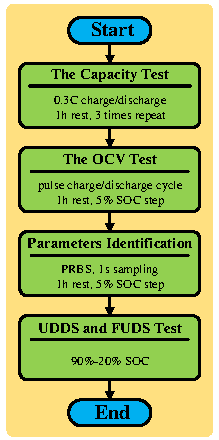
\includegraphics[scale=0.65]{images/Battery_Cell_Test_Scheme.pdf}
		\vspace{-2mm}
		\caption{Battery cell test scheme. \cite{Fazheng2019}}
	\end{figure}
	
\end{frame}


\begin{frame}
	
	\frametitle{SOC - OCP Relationship}
	
	Charging and discharging with C/3 capacity rate is taken
	into consideration for OCV-SOC calculation
	
	\begin{figure}
		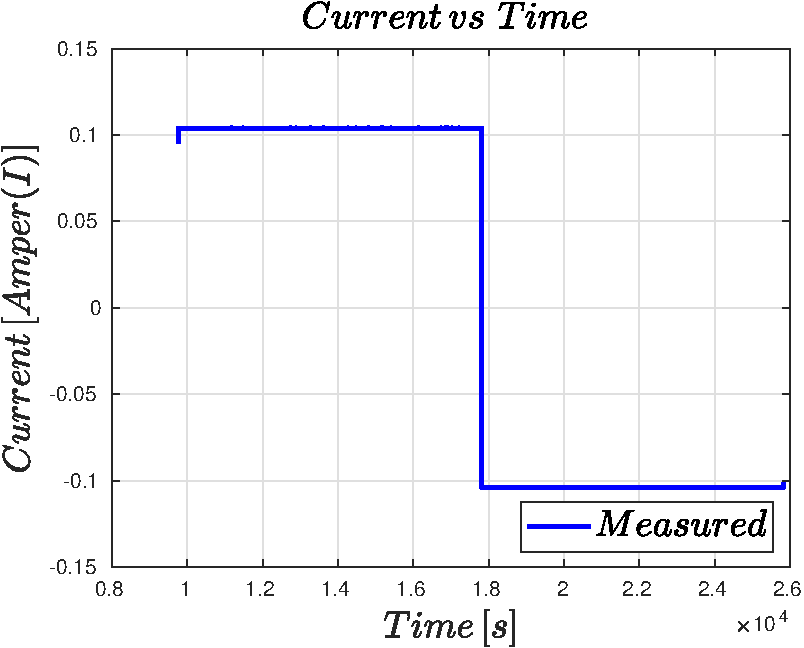
\includegraphics[scale=0.65]{images/OCV_vs_SOC_Current.pdf}
		\vspace{-2mm}
		\caption{Current measurement to obtain OCV-SOC Relation.}
	\end{figure}
	
\end{frame}


\begin{frame}
	
	\frametitle{SOC - OCP Relationship}
	
	Charging and discharging with C/3 capacity rate is taken
	into consideration to OCV-SOC relation:

	\begin{figure}
		\label{fig:OCV_vs_SOC}
		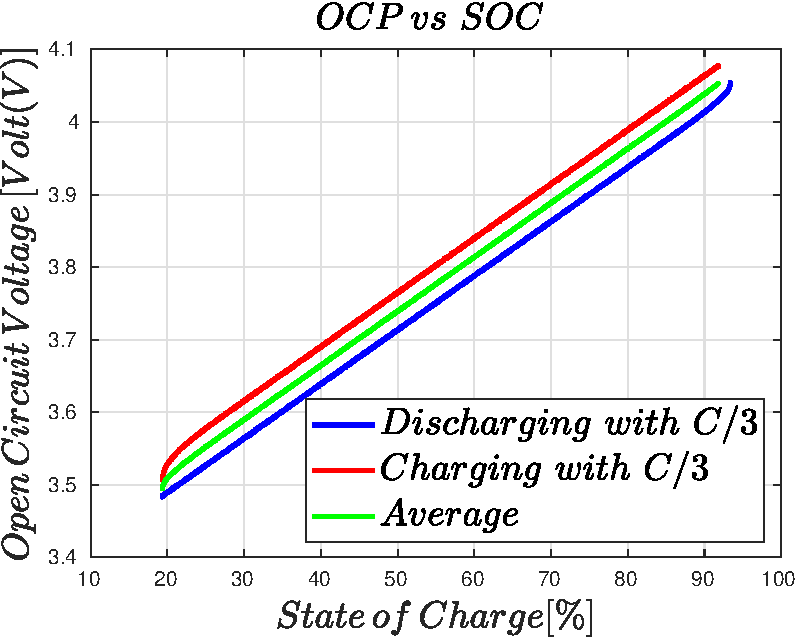
\includegraphics[scale=0.60]{images/OCV_vs_SOC.pdf}
		\vspace{-2mm}
		\caption{ Experimental SOC-OCV mapping when battery is charged/discharged with $C/3$ capacity.
			.}
	\end{figure}
	
\end{frame}


\begin{frame}
	
	\frametitle{SOC - OCP Models}
	
	\begin{table}[!b]
		\begin{tabular}{c | c | c } 
			\hline
			\# & Reference & RMS Error (mV)\\ [0.5ex] 
			\hline\hline
			$1$ &  \cite{Zhang2016} & $0.4798$ \\ 
			\hline
			$2$ &  \cite{Plett2004} & $0.2431$ \\ 
			\hline
			$3$ & \cite{Neumann2011} & $0.3060$ \\ 
			\hline
		\end{tabular}
		\caption{\label{table:Comparing_Fitting_Results}Compared fitting results of OCV models.}
	\end{table}
	
	\#1: $U_{OC}(s) = a  + b \times (-ln(s))^m + c \times s + d \times \exp^{n(s-1)}$ \\
	\#2: $U_{OC}(s) = K_{0} - \frac{K_{1}}{s} - K_{2}s + K_{3}ln(s) + K_{4}ln(1 - s)$ \\
	\#3: $U_{OC}(s) = K_{0} + K_{1}{\exp}^{-\alpha(1-s)} - \frac{K_{2}}{s}$ 
	
\end{frame}

\section{Parameters Identification of the Battery Model}

\begin{frame}
	
	\frametitle{Classification of the Identification Methods}
	
	\begin{figure}
		\centering
		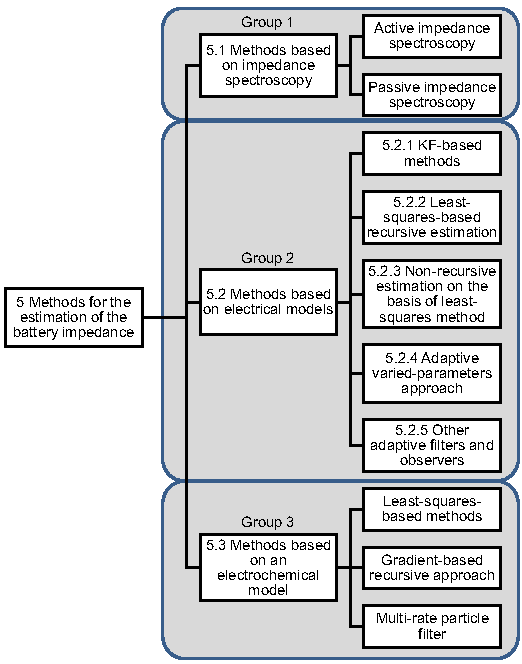
\includegraphics[height=0.60\textwidth, keepaspectratio]{images/Classification_of_the_methods_for_the_estimation_of_the_battery_impedance.pdf}
		\caption{Classification of the methods for the estimation of the battery parameters.\cite{WaaG2014}}
		\label{fig:Classification_of_the_methods_for_the_estimation_of_the_battery_impedance}
	\end{figure}
	
\end{frame}

\subsection{Preliminary Work}

\begin{frame}
	
	\frametitle{Preliminary Work}
	
	Before starting the parameter identification, continuous time dynamic equation  in \ref{eqn:continues_time_state_space}, i.e. $\dot{\bm{x}}(t) = \bm{A}\bm{x}(t)\,+\,\bm{B}u(t)$, must be discretized. \\
	
	$\bm{x} = [U_{1}\,\,U_{2}]^{T}$, and state transition matrix becomes $\bm{A} = \begin{bmatrix} -\frac{1}{R_{1}C_{1}} & 0 \\ 0 & -\frac{1}{R_{2}C_{2}} \end{bmatrix}$. Input matrix denoted as $\bm{B} = \begin{bmatrix} \frac{1}{C_{1}} \\ \frac{1}{C_{2}} \end{bmatrix}$.
	
	\begin{equation}
		\label{eqn:Solution_of_state_space equation_1}
		e^{-\bm{A}t}\dot{\bm{x}}(t) - e^{-\bm{A}t}\bm{A}\bm{x}(t) = \frac{d}{dt}\bigg(e^{-\bm{A}t}\bm{x}(t)\bigg)  = e^{-\bm{A}t}\bm{B}u(t)
	\end{equation}
	
	Solution is,
	\begin{subequations} 
		\label{eqn:Solution_of_state_space equation_3}
		\begin{align} 
			\bm{x}(t) &= e^{\bm{A}t}\bm{x}(0)  + e^{\bm{A}t}\int_{0}^{t} e^{-\bm{A}\tau}\bm{B}u(\tau)d\tau\\
			\bm{x}(t) &= e^{\bm{A}t}\bm{x}(0)  + \int_{0}^{t} e^{\bm{A}(t-\tau)}\bm{B}u(\tau)d\tau
		\end{align} 
	\end{subequations}
	
\end{frame}

\begin{frame}
	
	\frametitle{Preliminary Work cont'd}
	
	A continuous time signal $\{x(t)\}$ can be obtained from a discrete time (DT) signal ${x[k]}$:
	
	\begin{equation}
		\label{eqn:zero_order_hold}
		{x}(t) = x[k], \;\;\; kT \leq t < (k+1)T
	\end{equation}
	
	\begin{align}
		\begin{split}
			\bm{x}[k+1] &= \bm{A_{d}}\bm{x}[k] + \bm{B_{d}}u[k] \\
			y[k] &= \bm{C_{d}}\bm{x}[k] +  D_{d}u[k]
		\end{split}
	\end{align}

	 Starting from the solution of the continuous state-space equation \ref{eqn:Solution_of_state_space equation_3}
	
	\begin{equation}
		\label{eqn:discrete_system_matrices}
		\bm{A_d} = e^{\bm{A}T}\;\;\;\text{and}\;\;\;\bm{B_{d}}=\bigg(\int_{0}^{T}e^{A\tau}d\tau\bigg)\bm{B} 
	\end{equation}
	
	It should be note that that this is the \textit{exact} solution to the differential equation.

\end{frame}

\begin{frame}
	
	\frametitle{Preliminary Work cont'd}
	
	The discrete time dynamic equation can be explicity written as:
	
	\begin{equation}
		\label{eqn:discrete_state_space_matrix_form}
		\bm{x}[k+1] = \underbrace{\begin{bmatrix}
				e^{-\frac{Tt}{\tau_{1}}} & 0 \\
				0 & e^{-\frac{T}{\tau_{2}}} 
		\end{bmatrix}}_{\let\scriptstyle\textstyle\substack{\bm{A}_{d}}} \bm{x}[k] + \underbrace{\begin{bmatrix}
				R_{1}(1 - e^{\frac{T}{\tau_{1}}})  \\
				R_{2}(1 - e^{\frac{T}{\tau_{2}}})  
		\end{bmatrix}}_{\let\scriptstyle\textstyle\substack{\bm{B}_{d}}} u[k]
	\end{equation}

	where state vector is of the form $\bm{x}[k] = \big[U_{1}[k]\,\,U_{2}[k]\big]^{T}$, and input $u[k]$ is the measured current at each sampling time $I[k]$. And the continuous time matrices $\bm{C} = \bm{C_{d}}$ and $D=D_{d}$ remain same in discrete time.
	
	\begin{align}
		\label{eqn:discrete_state_space_equation_form}
		\begin{split}
			&U_{1}[k+1] = U_{1}[k]e^{-\frac{T}{\tau_{1}}} + I[k] R_{1}\big(1 - e^{\frac{T}{\tau_{1}}}\big) \\
			&U_{2}[k+1] = U_{2}[k]e^{-\frac{T}{\tau_{2}}} + I[k] R_{2}\big(1 - e^{\frac{T}{\tau_{2}}}\big)\\ 
			&U_{t}[k] = U_{OC}\big[SOC[k]\big] - I[k] R_{0} - U_{1}[k] - U_{2}[k]
		\end{split}
	\end{align}

\end{frame}

\subsection{Parameter Identification Procedure}

\begin{frame}
	
	\frametitle{Parameter Identification Based On Recursive Least Square\cite{Fazheng2019}}
	
	The transfer function of the second-order equivalent circuit model
	can be written as:
	
	\begin{equation}
		\label{eqn:transfer_function_Laplace_domain}
		G(s) = \frac{U_t(s) - U_{oc}(s)}{I(s)} = -\bigg(R_{0} + \frac{R_{1}}{1+\tau_{1}s} + \frac{R_{2}}{1+\tau_{2}s} \bigg)
	\end{equation}
	Transformation from ${L}$ (Laplace) domain to $z$ domain based on bilinear transformation:
	
	\begin{equation}
		\label{eqn:bilinear_transformation}
		s = \frac{2(1-z^{-1})}{T(1+z^{-1})}
	\end{equation}

	\begin{equation}
		\label{eqn:transfer_function_z_domain}
		G(z^{-1}) = \frac{\theta_{3} + \theta_{4}z^{-1} + \theta_{5}z^{-2}}{1-\theta_{1}z^{-1}-\theta_{2}z^{-2}}
	\end{equation}
	where parameters $\theta_{i} (i = 1, 2, ..., 5)$ being identified.
\end{frame}

\begin{frame}
	
	\frametitle{Parameter Identification Based On RLS cont'd}
	
	Let $y[k] = U_{t}[k] - U_{oc}[k]$, Equation \ref{eqn:transfer_function_z_domain} can be written as follows:
	
	\begin{equation}
		\label{eqn:discrete_output_equation}
		y[k] = \theta_{1}y[k-1] + \theta_{2}y[k-1] + \theta_{3}I[k] + \theta_{4}I[k-1] + \theta_{5}I[k-2]
	\end{equation}
	
	Defining $\bm{\phi}$ and new parameter vector, $\bm{\theta}$ as,
	
	\begin{equation}
		\label{eqn:RLS_psi_vector}
		\bm{\phi}[k] = \bigg[y[k-1]\,\,y[k-2]\,\,I[k]\,\,I[k-1]\,\,I[k-2]\bigg]^{T} 
	\end{equation}
	
	and
	
	\begin{equation}
		\label{eqn:RLS_theta_vector}
		\bm{\theta}[k] = \big[\theta_{1}\,\,\theta_{2}\,\,\theta_{3}\,\,\theta_{4}\,\,\theta_{5}\big]^{T} 
	\end{equation}
	
	Then Equation \ref{eqn:discrete_output_equation} can be written in vector form as follows:
	
	\begin{equation}
		\label{eqn:discrete_output_equation_2}
		y[k] = \bm{\phi}[k]^{T}\bm{\theta}[k]
	\end{equation}
	
\end{frame}


\begin{frame}
	
	\frametitle{Parameter Identification Based On RLS cont'd}
	
	Defining the estimator of $\bm{\theta}$ as $\bm{\hat{\theta}}$, Equation \ref{eqn:discrete_output_equation_2} can be expressed as:
	
	\begin{equation}
		\label{eqn:discrete_output_equation_3}
		y[k] = \bm{\phi}[k]^{T}\bm{\hat{\theta}}[k] + \varepsilon[k]
	\end{equation}	
	
	When the square sum of ε the output error is minimum, the parameters are optimal, and the mathematical formula can be written as
	
	\begin{equation}
		\label{eqn:RLS}
		\underset{\bm{\hat{\theta}}}{\text{min}}
		\,\,\bm{{J}}(\bm{\hat{\theta}},k) = \underset{\bm{\hat{\theta}}}{\text{min}} \sum_{k=k_{0}}^{N}\varepsilon[k]^{2} = \underset{\bm{\hat{\theta}}}{\text{min}} \sum_{k=k_{0}}^{N}\bigg(y[k] - \bm{\phi}[k]^{T}\bm{\hat{\theta}}[k]\bigg)^{2}
	\end{equation}
	
	\begin{equation}
		\label{eqn:Least_square_one_step_solution}
		\bm{\hat{\theta}} = (\bm{\Psi}^{T}\bm{\Psi})^{-1}\bm{\Psi}^{T}\bm{Y}
	\end{equation}

	where vectors compose of past measurements $\bm{\Psi}= \big[\bm{\phi}[k_{0}]\,\,\bm{\phi}[k_{0}+1]\,\,\dots\,\,\bm{\phi}[N]\big]^{T}$ and big output vector $\bm{Y}=\big[y[k_{0}]\,\,y[k_{0}+1]\,\,\dots\,\,y[N]\big]^{T}$.
	
\end{frame}

\subsubsection{The Parameter Estimation Algorithm}

\begin{frame}
	
	\frametitle{The Measurement of Current and Terminal Voltage For Estimation Algorithm}
	
	\begin{figure}
		\centering
		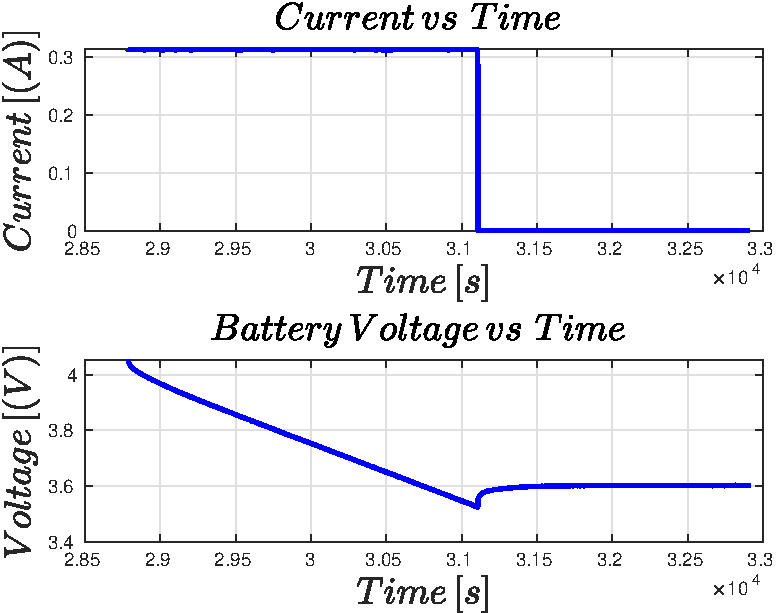
\includegraphics[width=0.8\textwidth, keepaspectratio]{images/Parameter_Identification_Region.pdf}
		\caption{Measurement of current and voltage
			from a pulse response for second order equivalent circuit parameters identification.}
		\label{fig:Response_to_discharge_pulse_experimental}
	\end{figure}
	
\end{frame}

\begin{frame}
	
	\frametitle{Identified Parameters}
	
	\begin{figure}
		\centering
		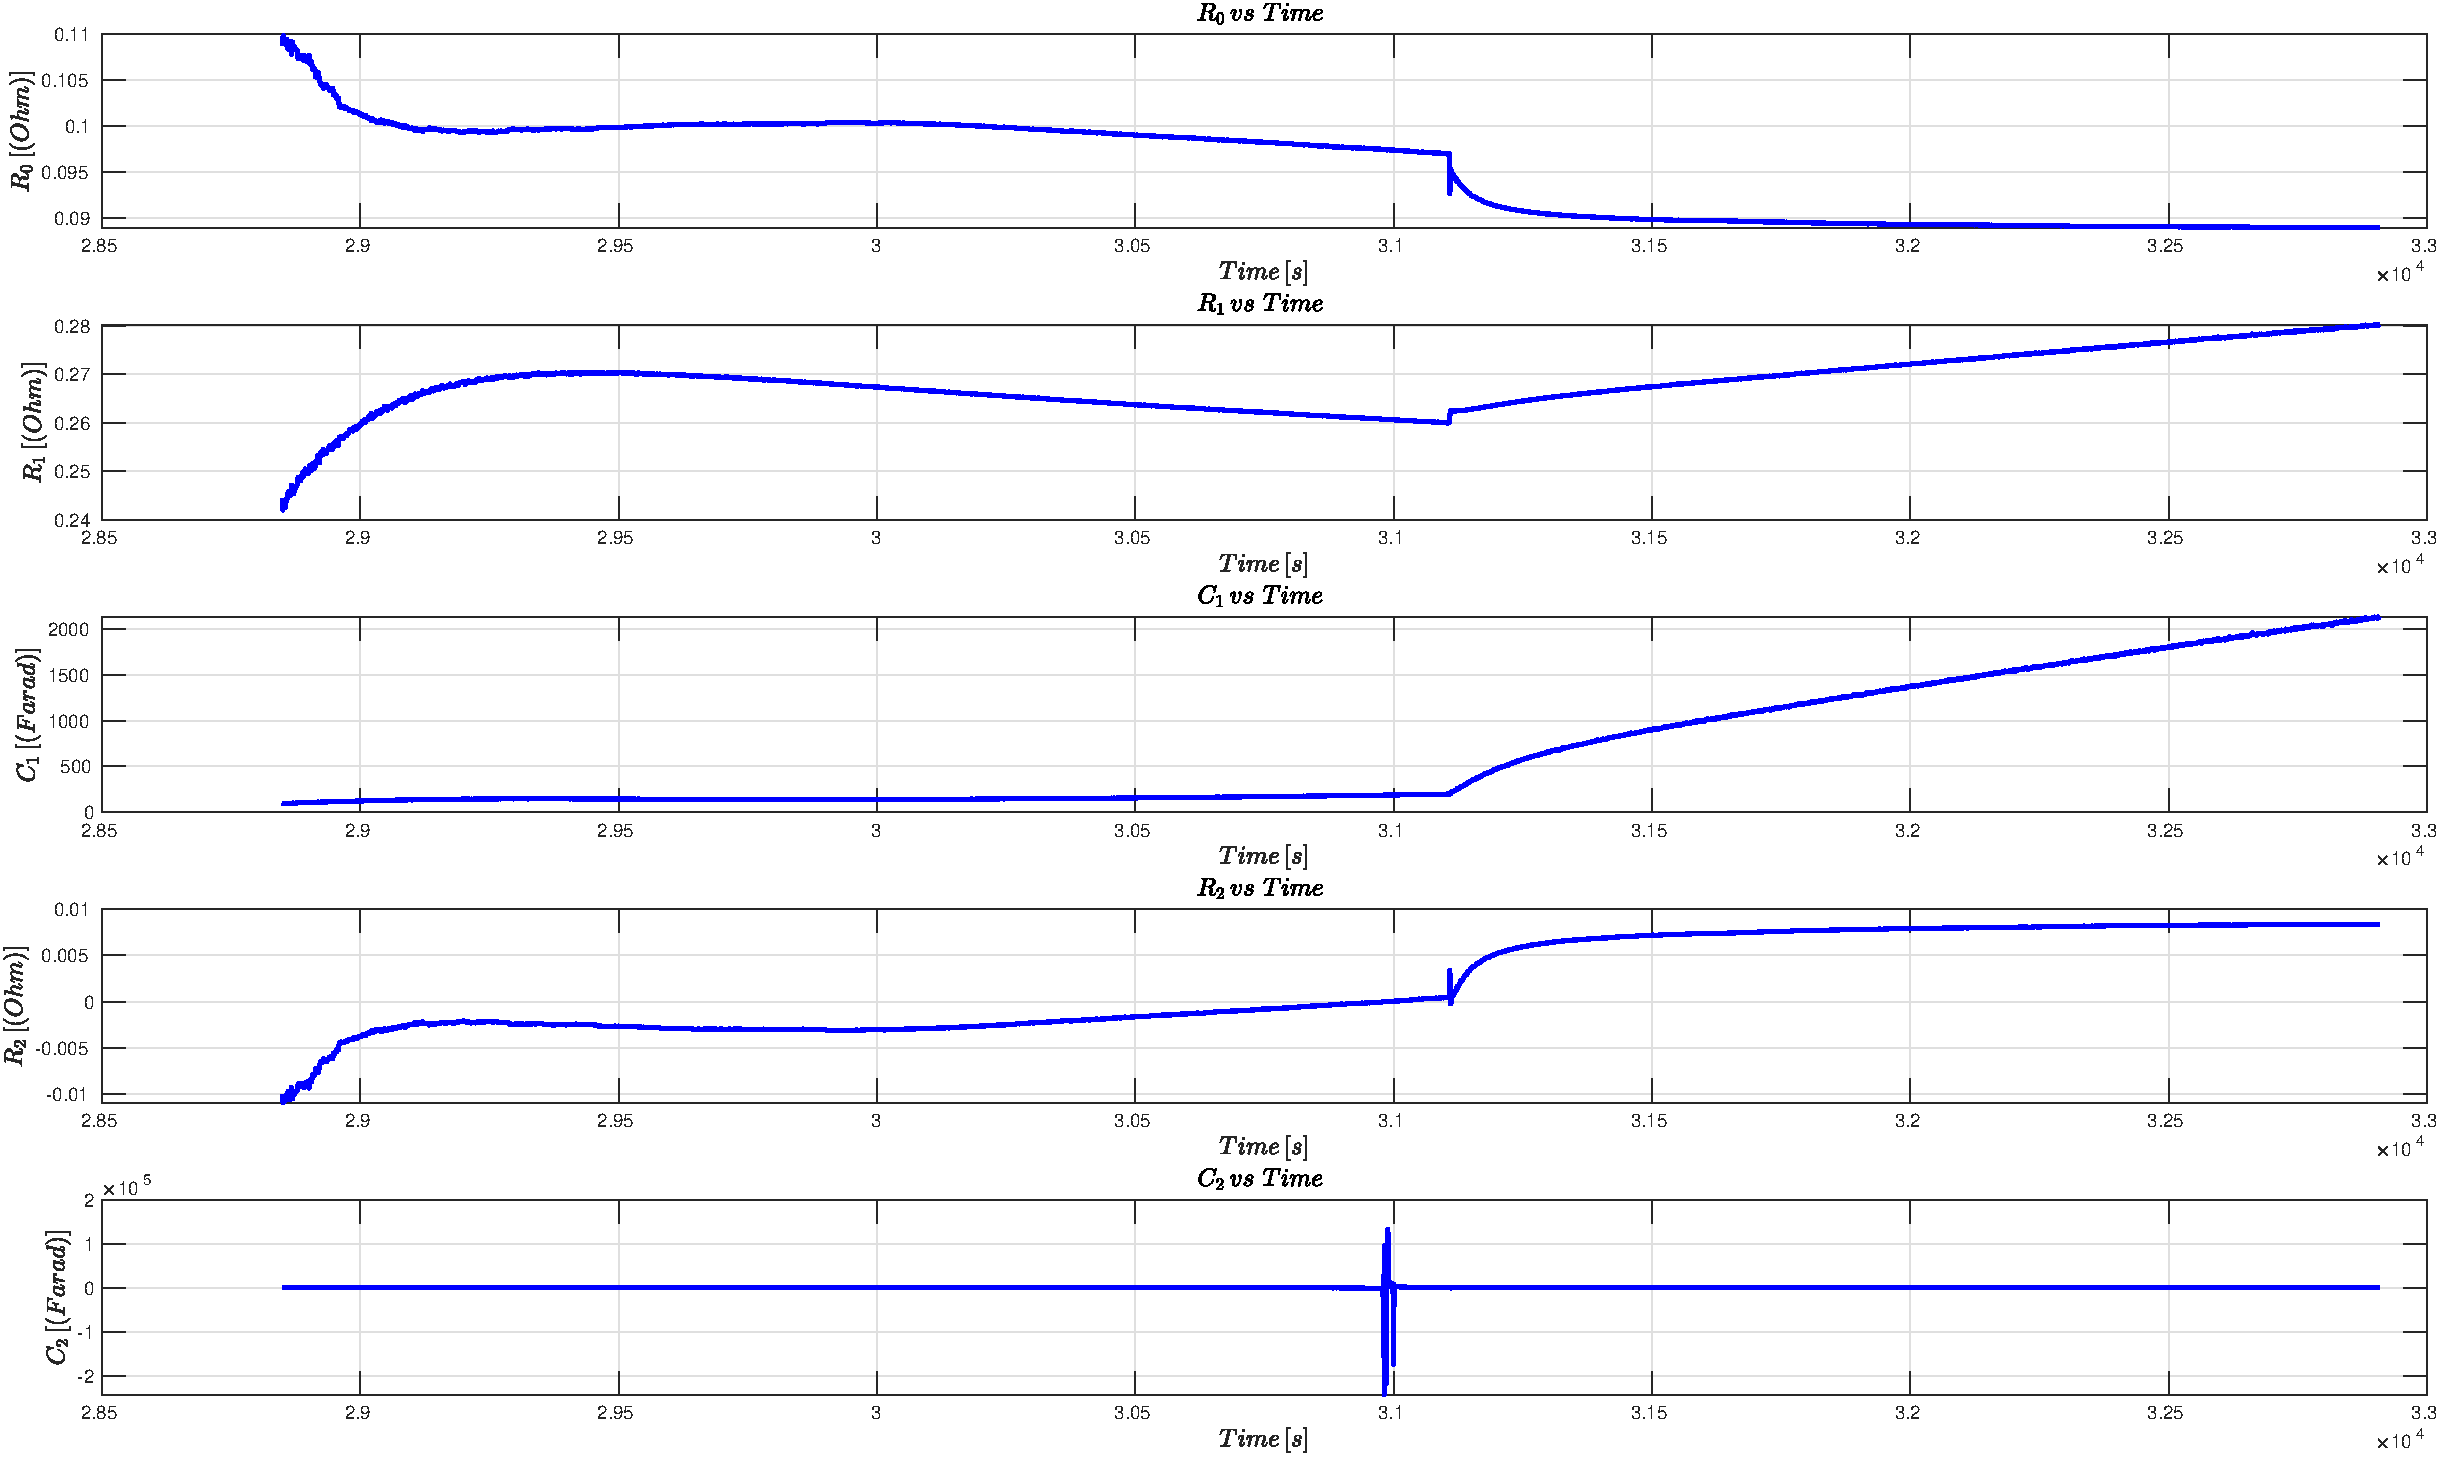
\includegraphics[width=\textwidth, keepaspectratio]{images/RLS_Results.pdf}
		\caption{Parameter identification results of the RLS algorithm for parameters $R_{0}$, $R_{1}$, $R_{2}$, $C_{1}$ and $C_{2}$.}
		\label{fig:Results_of_the_RLS_Method}
	\end{figure}	
\end{frame}

\section{SOC Estimation} 
\label{SOC_Estimation}

\begin{frame}
	
	\frametitle{SOC Estimation}
	
	\begin{figure}
		\centering
		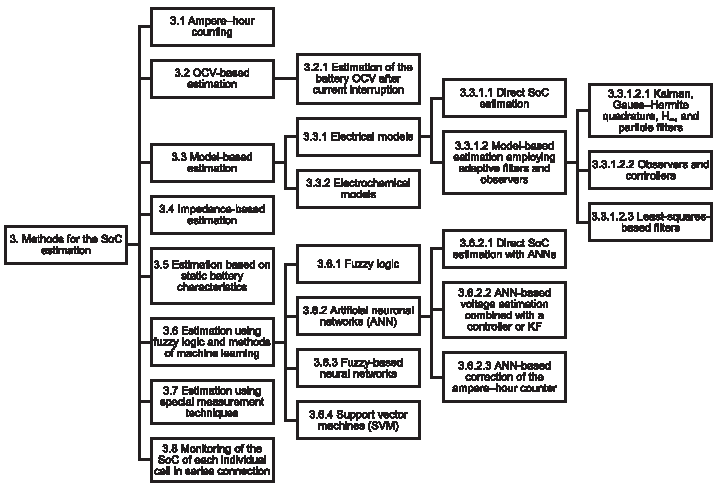
\includegraphics[width=0.9\textwidth, keepaspectratio]{images/Classification_of_the_methods_for_the_SoC_estimation.pdf}
		\caption{Classification of the methods for the SOC estimation. \cite{WaaG2014}}
		\label{fig:Classification_of_the_methods_for_the_SOC_estimation}
	\end{figure}
	
\end{frame}

\subsection{Adaptive EKF Algorithm}
\label{Adaptive_EKF}

\begin{frame}
	
	\frametitle{Adaptive EKF}
	
	Reform a state-space form in Equation \ref{eqn:discrete_state_space_matrix_form}: 
	
	\begin{align}
		\label{eqn:discrete_state_space_matrix_form_for_EKF_1}
		\begin{split}
			\bm{x}[k+1] &= f(\bm{x[k]},u[k]) =\bm{A_{d}}\bm{x}[k] + \bm{B_{d}}u[k] + \bm{w}[k]\\
			y[k] &= h(\bm{x[k]},u[k]) + v[k]
		\end{split}
	\end{align}
	
	Explicity,
	
	\begin{equation}
		\label{eqn:discrete_state_space_matrix_form_for_EKF_2}
		\bm{x}[k+1] = \underbrace{\begin{bmatrix}
				e^{-\frac{Tt}{\tau_{1}}} & 0 & 0\\
				0 & e^{-\frac{T}{\tau_{2}}} & 0 \\
				0 & 0 & 1
		\end{bmatrix}}_{\let\scriptstyle\textstyle\substack{\bm{A}_{d}}} \bm{x}[k] + \underbrace{\begin{bmatrix}
				R_{1}(1 - e^{\frac{T}{\tau_{1}}})  \\
				R_{2}(1 - e^{\frac{T}{\tau_{2}}})  \\
				-\frac{\eta T}{Q}
		\end{bmatrix}}_{\let\scriptstyle\textstyle\substack{\bm{B}_{d}}} u[k]
		+ \bm{w}[k]
	\end{equation}
	
	The state vector with SOC is denoted by $\bm{x}[k] = \bigg[U_{1}[k]\,\,U_{2}[k]\,\,SOC[k]\bigg]^{T}$. $\bm{w}[k] \sim {N}(0,\,\bm{Q})$ is the unmeasured process noise, $v[k] \sim {N}(0,\,\bm{R})$ is the measurement noise.
	
\end{frame}

\begin{frame}
	
	\frametitle{Adaptive EKF}
	
	The matrix $\bm{C}$ is the derivative of the output equation (\ref{eqn:discrete_state_space_matrix_form_for_EKF_1}) w.r.t. state vector before estimation time, $\bm{C}[k]= \dfrac{\partial h(\bm{x}[k],u[k])}{\partial \bm{x}}\Biggr|_{\substack{x=\hat{x}[k]^{-}}} = \bigg[-1\,-1\,\dfrac{dU_{oc}(SOC)}{dSOC}\Bigr|_{\substack{\hat{SOC}[k]^{-}}}\bigg]$ where $\dfrac{dU_{oc}(SOC)}{dSOC} = K_{1}SOC^{-2}-K_{2}+ \dfrac{K_{3}}{SOC}-\dfrac{K_{4}}{1-SOC}$.
	
	\vspace{-2mm}
	
	\begin{figure}
		\centering
		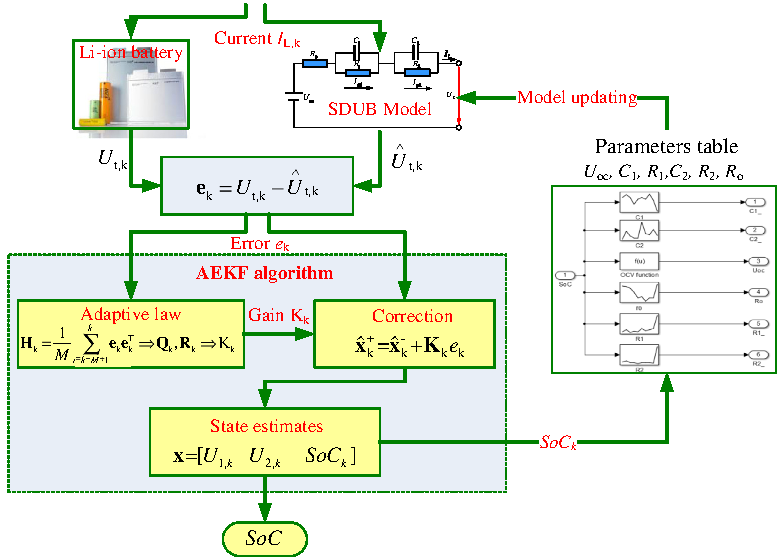
\includegraphics[height=0.45\textwidth, keepaspectratio]{images/Data_Driven_SoC_Estimation_Approach_With_AEKF_Algorithm.pdf}
		\caption{The implementation flowchart of the data driven-based SoC estimation approach with AEKF algorithm. }
		\label{fig:AEKF_Algorithm_Flowchart}
	\end{figure}
	
\end{frame}

\begin{frame}
	
	\frametitle{Adaptive EKF Algorithm}
	
	\begin{figure}
		\centering
		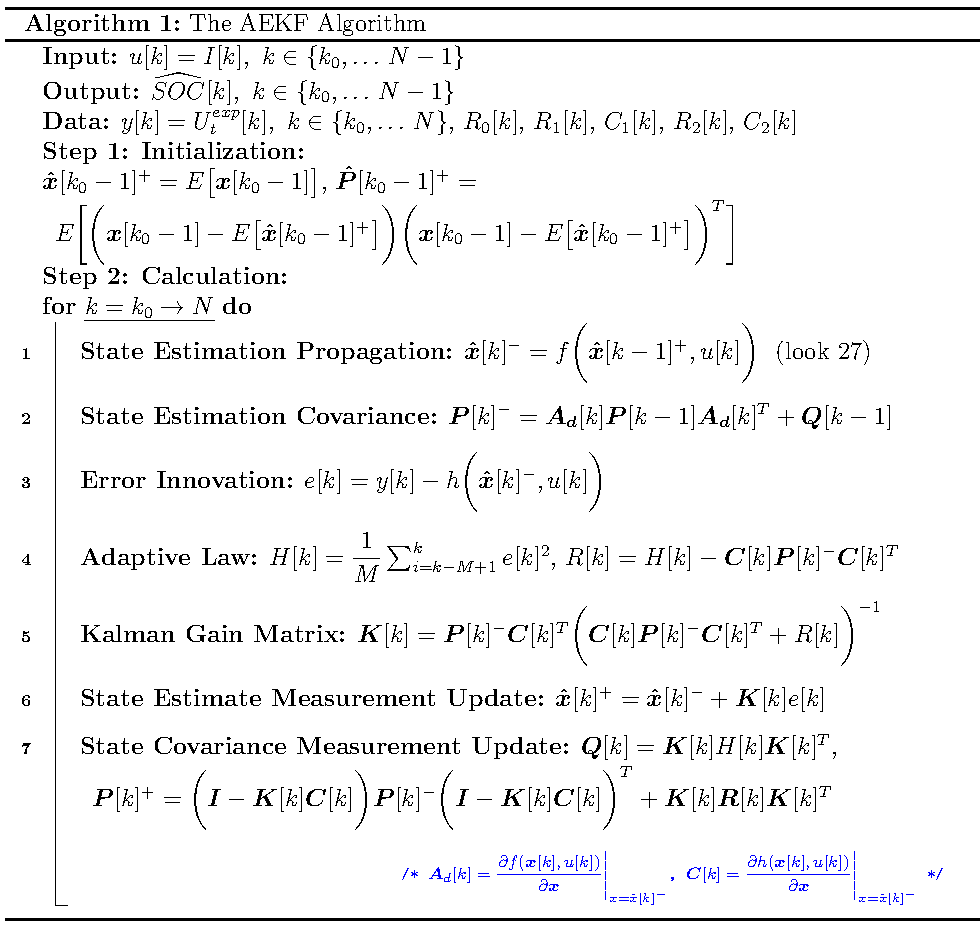
\includegraphics[height=0.75\textwidth, keepaspectratio]{images/AEKF_Algorithm.pdf}
		%\caption{The implementation flowchart of the data driven-based SoC estimation approach with AEKF algorithm. }
		\label{fig:AEKF_Algorithm}
	\end{figure}
	
\end{frame}

\section{Results of The SOC Estimation and The Parameter Identification}

\begin{frame}
	
	\frametitle{Estimated SOC vs Time}
	
	\begin{figure}
		\centering
		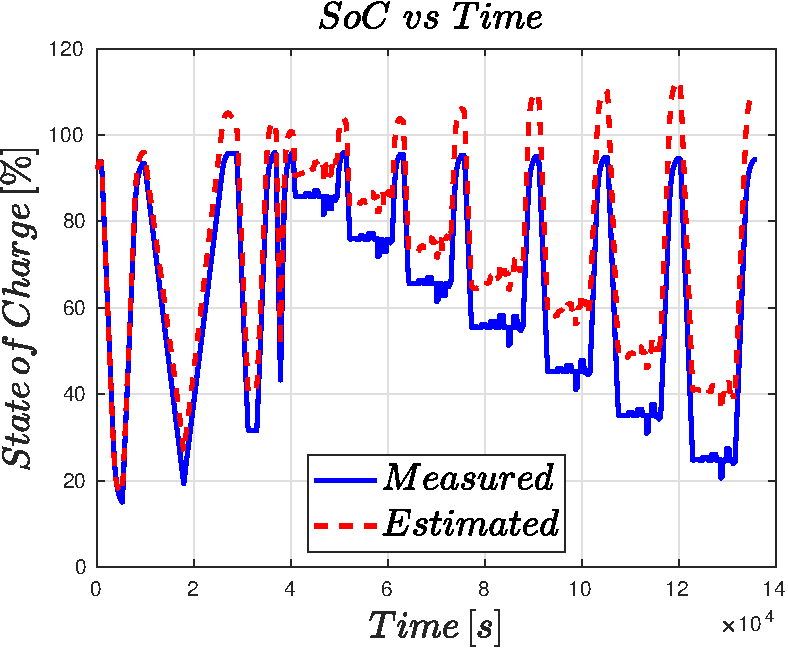
\includegraphics[width=0.7\textwidth, keepaspectratio]{images/AEKF_SOC.pdf}
		\caption{Validation results for SOC estimation by using AEKF.}
		\label{fig:The_AEKF_SOC}
	\end{figure}
	
\end{frame}

\begin{frame}
	
	\frametitle{Estimated Terminal Battery Voltage , $U_{t}$,  vs Time}
	
	\begin{figure}
		\centering
		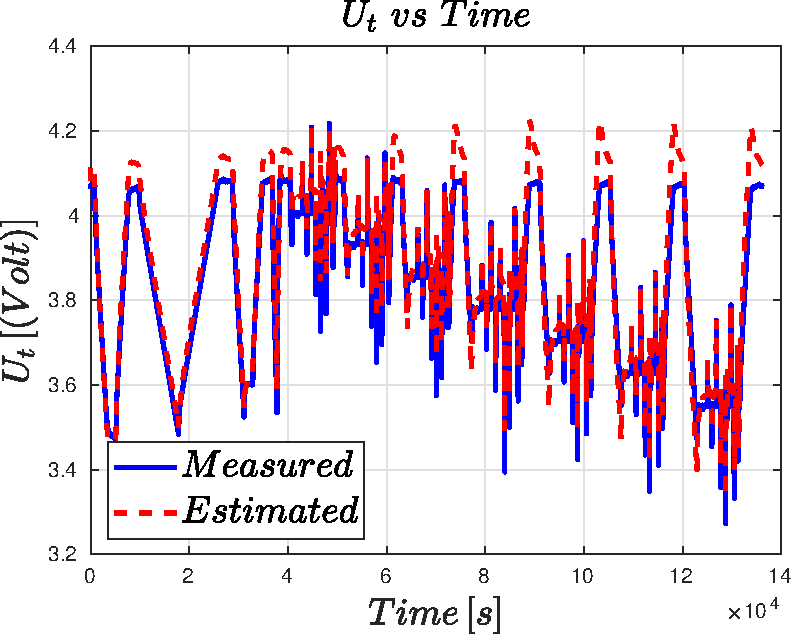
\includegraphics[width=0.7\textwidth, keepaspectratio]{images/AEKF_Terminal_Voltage.pdf}
		\caption{Validation results for terminal voltage, $U_{t}$, by using AEKF}
		\label{fig:The_AEKF_Terminal_Voltage}
	\end{figure}
	
\end{frame}


\begin{frame}
	
	\frametitle{Terminal Battery Voltage Error, $e_{t}$,  vs Time}
	
	\begin{figure}
		\centering
		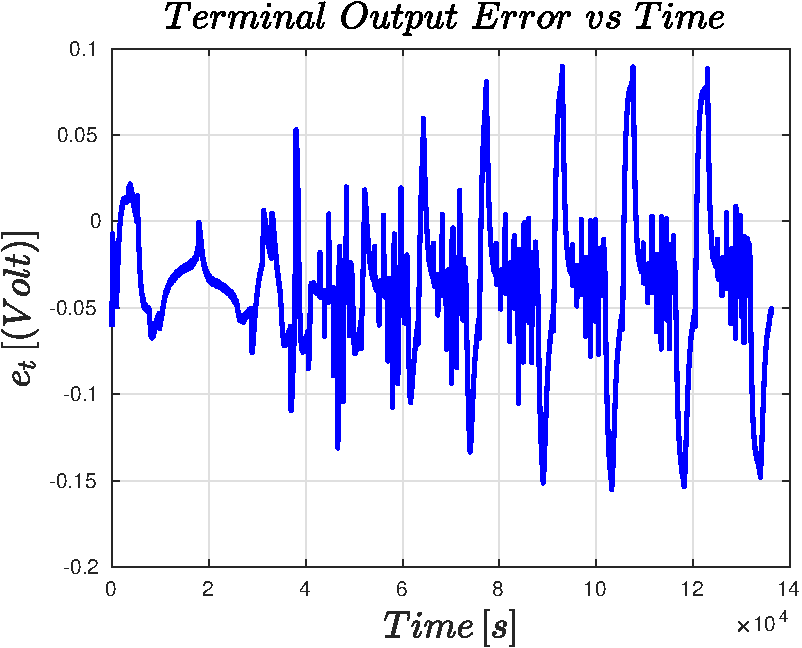
\includegraphics[width=0.7\textwidth, keepaspectratio]{images/AEKF_Terminal_Voltage_Error.pdf}
		\caption{Error between estimated battery terminal voltage and  terminal voltage, $U_{t}$, by using AEKF}
		\label{fig:The_AEKF_Terminal_Voltage_Error}
	\end{figure}
	
\end{frame}

\begin{frame}
	
	\frametitle{State estimation for RC voltages vs Time}
	
	\begin{figure}
		\centering
		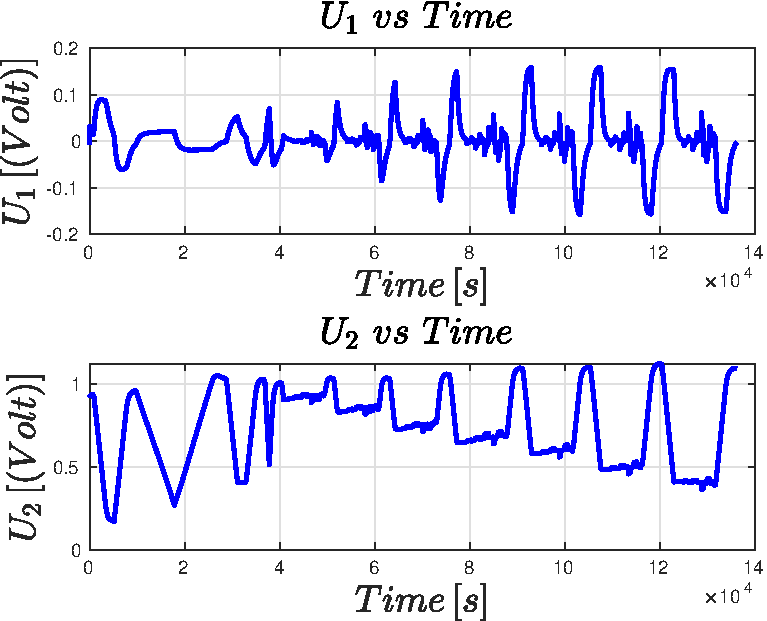
\includegraphics[width=0.7\textwidth, keepaspectratio]{images/AEKF_RC_Voltages.pdf}
		\caption{AEKF's state estimation for RC voltages $U_{1}$ and $U_{2}$, respectively }
		\label{fig:The_AEKF_RC_Voltages}
	\end{figure}
\end{frame}

\begin{frame}
	
	\frametitle{Estimated Parameters by using RLS}
	
	\begin{figure}
		\centering
		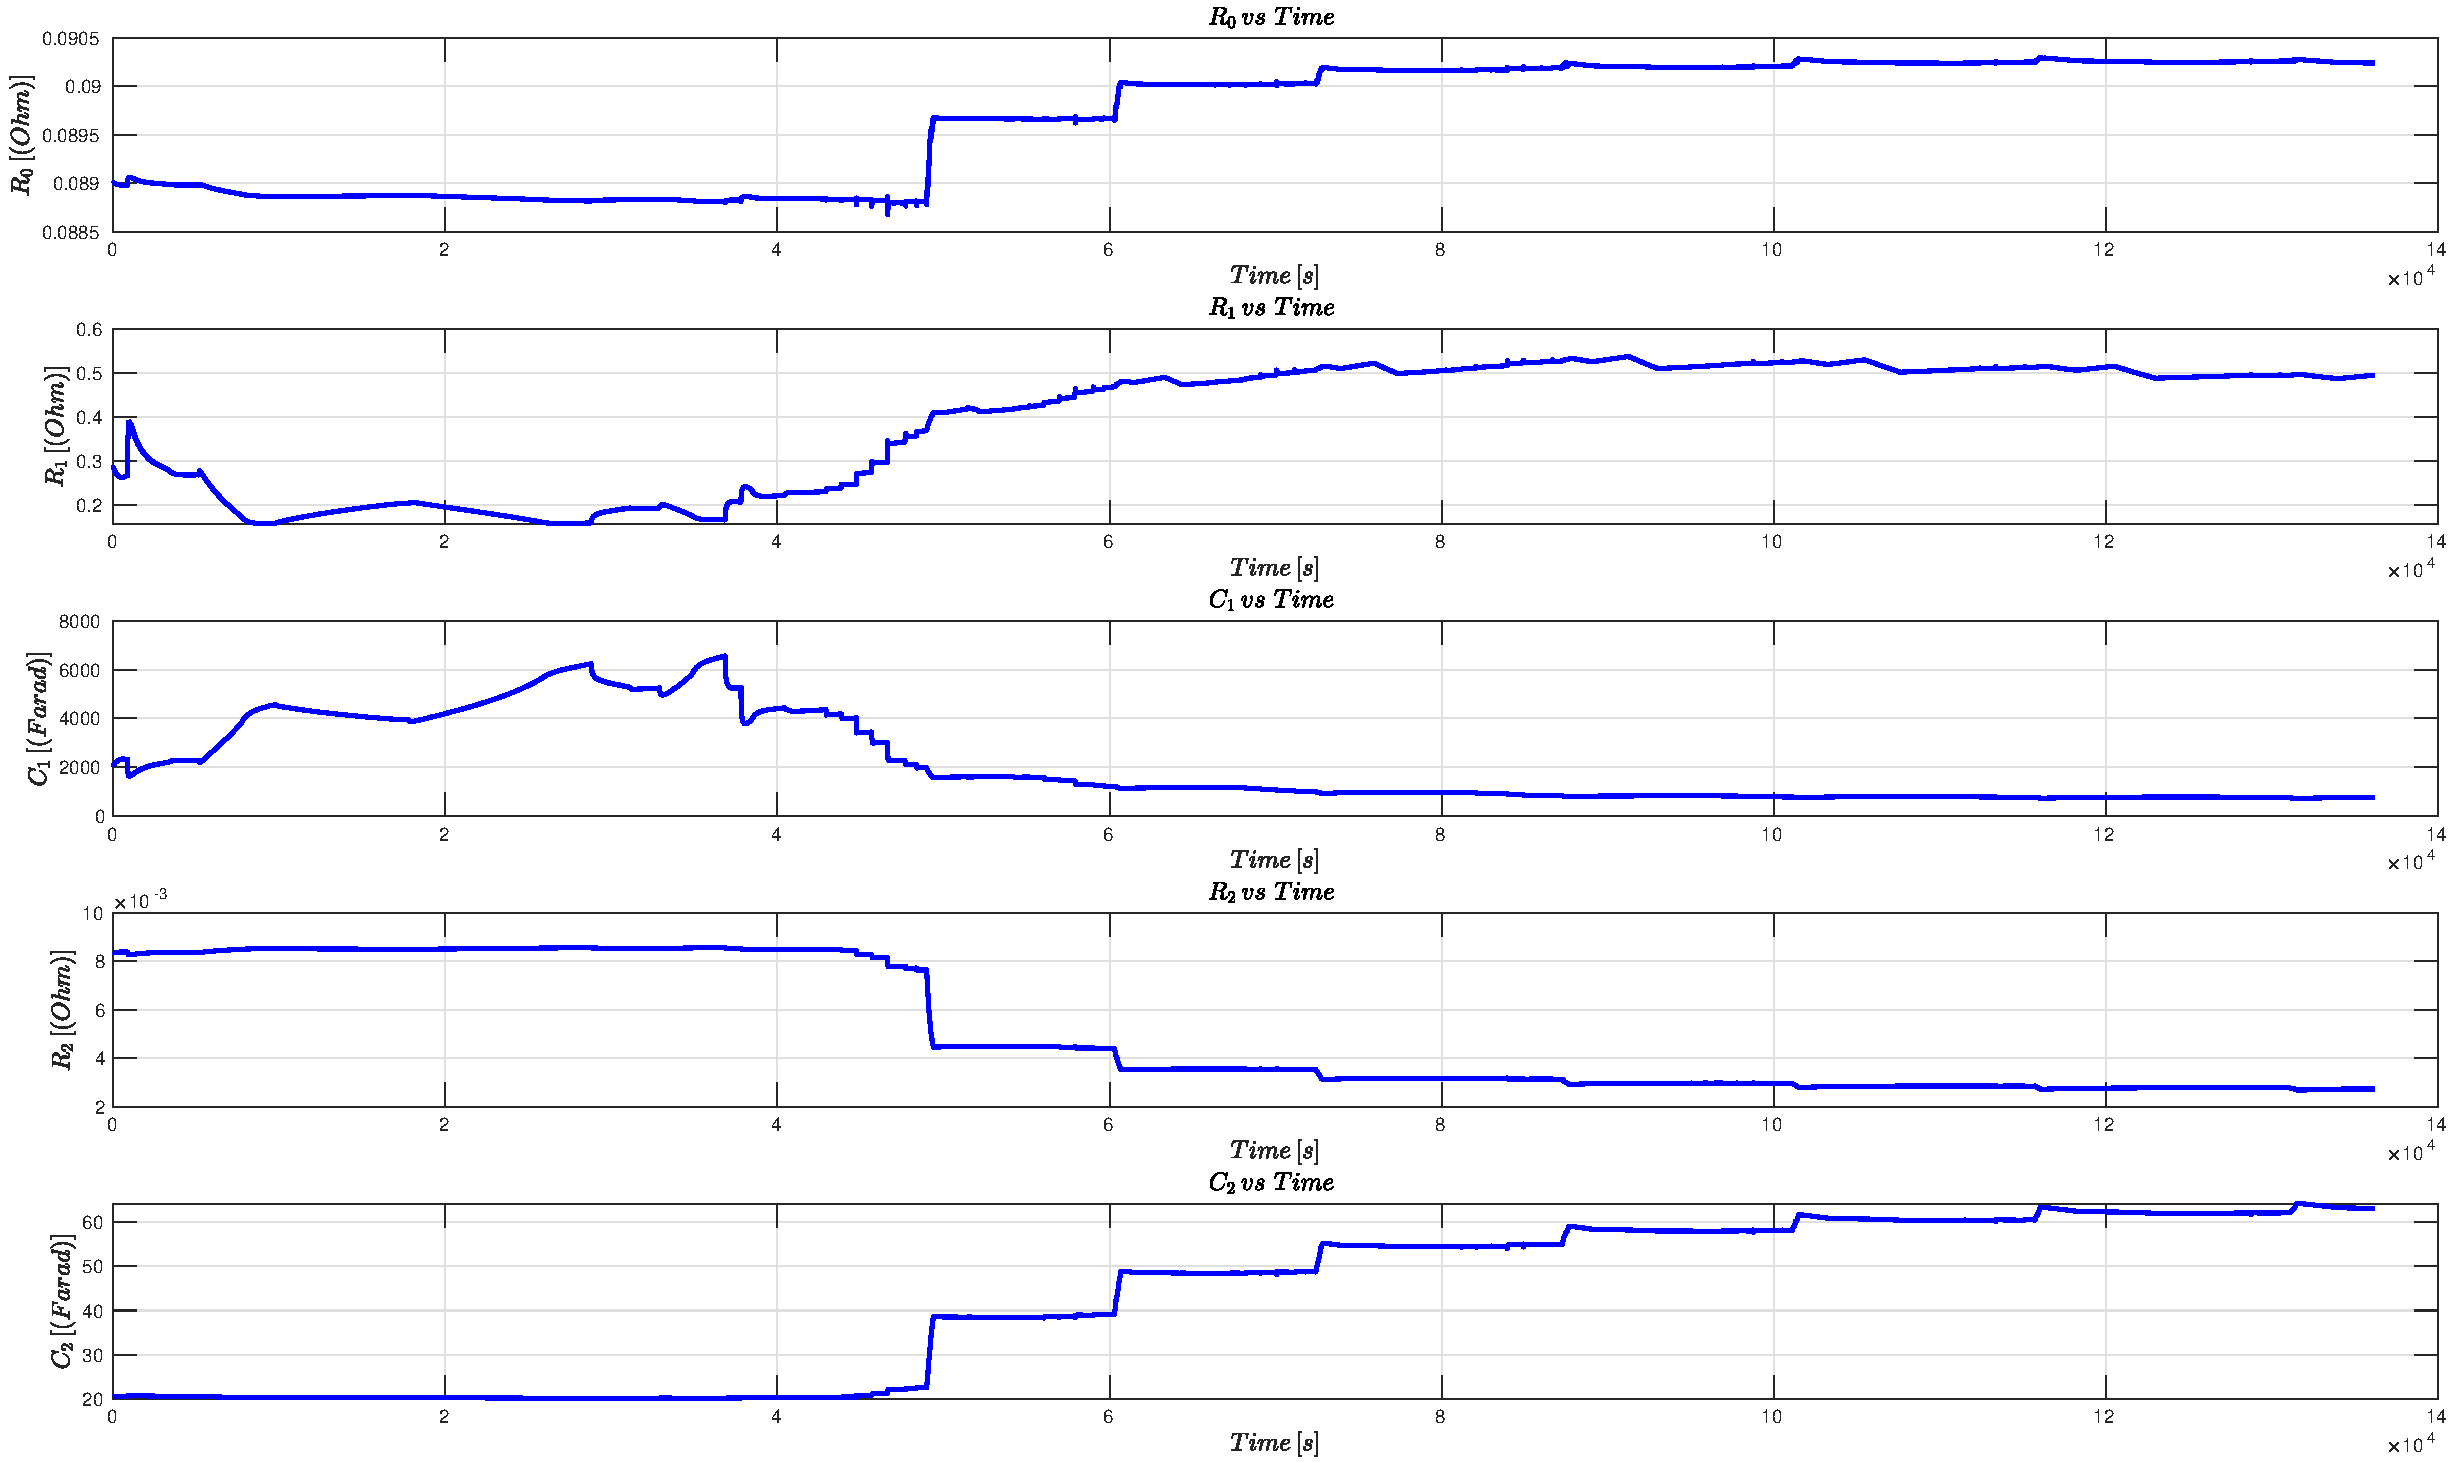
\includegraphics[width=1.0\textwidth, keepaspectratio]{images/RLS_Results_With_AEKF.pdf}
		\caption{Estimated Parameters by using RLS through whole experiment time.}
		\label{fig:RLS_Results_With_AEKF}
	\end{figure}
\end{frame}


%\begin{frame}{}
%	\centering \huge
%	Thank you for your attention! Any Question?
%\end{frame}

\end{document}
